
\begin{figure}
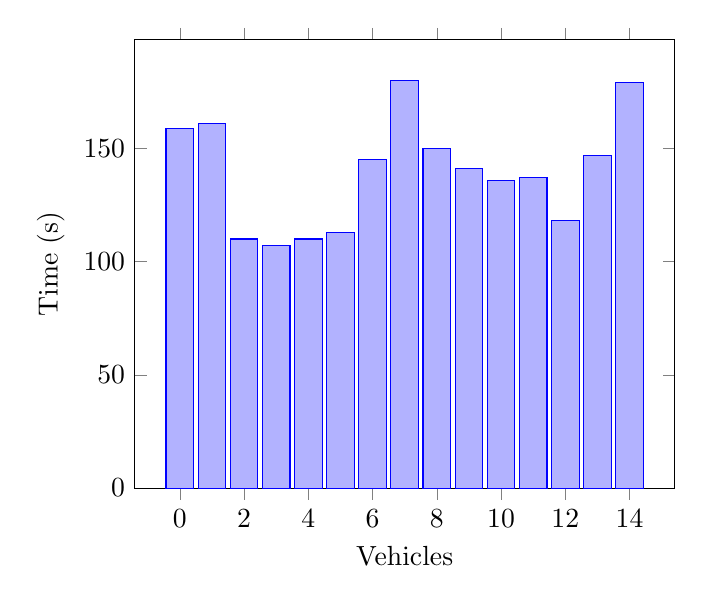
\begin{tikzpicture}
\begin{axis}[
legend style={anchor=west},
xlabel=Vehicles,
ylabel=Time (s),
ymin=0,
ybar,
]
\addplot coordinates {
(0, 159)
(1, 161)
(2, 110)
(3, 107)
(4, 110)
(5, 113)
(6, 145)
(7, 180)
(8, 150)
(9, 141)
(10, 136)
(11, 137)
(12, 118)
(13, 147)
(14, 179)
};

\end{axis}
\end{tikzpicture}
\label{tik:100:19_O, 19_O.-60, 17_N, 15_S, 15_S.-30, 13_N, 13_N.-40, 11_N, 8_N, 7_N, 7_N.-60, 5_N, 4_N, 4_N.-60, 3_O}
\caption{100 percent diving with GSC on route $19_O, 19_O.-60, 17_N, 15_S, 15_S.-30, 13_N, 13_N.-40, 11_N, 8_N, 7_N, 7_N.-60, 5_N, 4_N, 4_N.-60, 3_O$}
\end{figure}
